%=======================================================================
%  CH 7 — NUMERICAL PROBLEMS & SOLUTIONS
%=======================================================================
\section*{\color{acc}Ch 7 --- Advanced Applications --- Numerical Problems \& Solutions}
\vspace{-4pt}{\color{acc}\rule{\textwidth}{1.1pt}}\vspace{4pt}

{\color{sub}\footnotesize This chapter is almost entirely short notes. Across all 23 papers there is
exactly \textbf{one} numerical \yr{76 Ch}, on PageRank. It is solved in full below, plus 1 practice
problem on the variant most likely to be set next.}

\hr

%=======================================================================
\T{M1. PageRank}

\lead{Method}
\[ PR(A) = (1-d) + d\sum_{i}\frac{PR(T_i)}{C(T_i)} \]
\begin{enumerate}
  \item \textbf{Write down the link table first}: for every page, its \textbf{outlinks} (to get
        $C$) and its \textbf{inlinks} (to know which terms to sum). \mk{Nearly every error comes
        from confusing the two.}
  \item Initialise all ranks (here 0.25).
  \item Each iteration, compute all pages using the \textbf{previous} iteration's values, then
        substitute in together.
  \item Repeat for the required number of iterations, or until the values settle.
\end{enumerate}
\begin{itemize}
  \item \mk{A page's own rank is split equally among its outlinks} --- that is the $/C(T_i)$.
  \item A page with \textbf{no inlinks} sits permanently at $(1-d) = 0.15$.
\end{itemize}

\creamq{Problem 1.1}{\m{8}}
\begin{asked}{2076 Chaitra \textperiodcentered{} Q12 \textperiodcentered{} [8]}
\sbsr{0.56}{%
Consider the following subset of pages and their links. Apply the PageRank algorithm using a
damping factor of 0.85. A minimum of five iterations are required. Assume initial page rank of
all pages is 0.25.}{%
\vspace{0pt}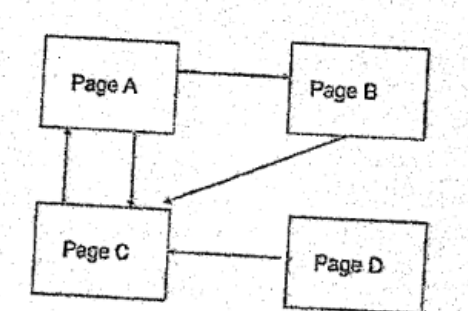
\includegraphics[width=0.86\linewidth]{figs/pyq_pagerank_76ch}}
\end{asked}

\sbs{%
\lead{Step 1: read the graph}
\begin{tabularx}{\linewidth}{@{}L{1.5cm}XL{1.2cm}X@{}}
\toprule
\hrow \thead{Page} & \thead{Outlinks} & \thead{$C$} & \thead{Inlinks} \\
A & B, C & \textbf{2} & C \\
B & C & \textbf{1} & A \\
C & A & \textbf{1} & A, B, D \\
D & C & \textbf{1} & \mk{none} \\
\bottomrule
\end{tabularx}
\lead{Step 2: write the 4 equations} ($d = 0.85$, $1-d = 0.15$)
\begin{itemize}
  \item $PR(A) = 0.15 + 0.85\,PR(C)$
  \item $PR(B) = 0.15 + 0.85\,\dfrac{PR(A)}{2}$
  \item $PR(C) = 0.15 + 0.85\Big(\dfrac{PR(A)}{2} + PR(B) + PR(D)\Big)$
  \item $PR(D) = 0.15 + 0.85(0) = \mathbf{0.15}$ \ \mk{constant, D has no inlinks}
\end{itemize}
\begin{itemize}
  \item Note $A$'s rank is divided by 2 because A links to \emph{both} B and C.
\end{itemize}}{%
\lead{Step 3: iterate}
\begin{tabularx}{\linewidth}{@{}L{1.2cm}XXXX@{}}
\toprule
\hrow \thead{Iter} & \thead{PR(A)} & \thead{PR(B)} & \thead{PR(C)} & \thead{PR(D)} \\
0 & 0.2500 & 0.2500 & 0.2500 & 0.2500 \\
1 & 0.3625 & 0.2563 & 0.6813 & 0.1500 \\
2 & 0.7291 & 0.3041 & 0.6494 & 0.1500 \\
3 & 0.7020 & 0.4599 & 0.8459 & 0.1500 \\
4 & 0.8690 & 0.4484 & 0.9668 & 0.1500 \\
\textbf{5} & \textbf{0.9718} & \textbf{0.5193} & \textbf{1.0280} & \textbf{0.1500} \\
\bottomrule
\end{tabularx}
{\color{sub}\footnotesize Row 0 is the given start value.}
\lead{Sample working (iteration 1)}
\begin{itemize}
  \item $PR(A) = 0.15 + 0.85(0.25) = 0.3625$
  \item $PR(B) = 0.15 + 0.85(0.25/2) = 0.2563$
  \item $PR(C) = 0.15 + 0.85(0.125+0.25+0.25) = 0.6813$
  \item $PR(D) = 0.15$
\end{itemize}}

\lead{Final answer after 5 iterations}
\begin{itemize}
  \item $PR(A)=0.972$, \ $PR(B)=0.519$, \ $PR(C)=1.028$, \ $PR(D)=0.150$
  \item \textbf{Ranking}: \mk{C $>$ A $>$ B $>$ D}
\end{itemize}

\begin{center}\fbox{\begin{minipage}{0.92\textwidth}\small
\mk{Two comments worth writing, they show understanding.} \added \\
\textbf{1.} The values are still climbing at iteration 5 but the \textbf{ranking has been stable
since iteration 3}. PageRank converges on \emph{order} much faster than on \emph{value}, which is
why 5 iterations is enough for the question. \\
\textbf{2.} Solving the equations exactly gives the fixed point
$PR(A)=1.490$, $PR(B)=0.783$, $PR(C)=1.577$, $PR(D)=0.150$, and these sum to
$\mathbf{4.00} = N$. \textbf{That sum is your check} --- in this (non-normalised) form the ranks
always converge to the number of pages. \\
\textbf{3.} \textbf{C wins} because it collects links from three pages while A collects only one,
and \textbf{D is stuck at 0.15} because nothing points to it. Linking out never raises your own rank.
\end{minipage}}\end{center}

\creamq{Practice --- the normalised form}{}
\begin{asked}[PROBLEM]{not a PYQ \textperiodcentered{} the same graph, normalised form \added}
Repeat Problem 1.1 on the same four-page graph, but using the \emph{normalised} PageRank
formula
\[ PR(A) = \frac{1-d}{N} + d\sum_i \frac{PR(T_i)}{C(T_i)} \]
with $d = 0.85$, $N = 4$ and an initial rank of 0.25 for every page. Compare the converged
ranks and the ordering with those of Problem 1.1.
\end{asked}
{\color{sub}\footnotesize This form makes the ranks sum to \textbf{1} instead of $N$.
Know both. \added}

\begin{itemize}
  \item With $N=4$, $\frac{1-d}{N} = \frac{0.15}{4} = 0.0375$.
  \item Iteration 1 from the same 0.25 start:
  \begin{itemize}
    \item $PR(A) = 0.0375 + 0.85(0.25) = 0.2500$
    \item $PR(B) = 0.0375 + 0.85(0.125) = 0.1438$
    \item $PR(C) = 0.0375 + 0.85(0.625) = 0.5688$
    \item $PR(D) = 0.0375$
  \end{itemize}
  \item Sum $= 1.0001 \approx 1$ \checkmark \ --- \mk{that is the check for this form.}
  \item \textbf{The ranking is identical} (C $>$ A $>$ B $>$ D); only the scale differs.
  \item \mk{In the exam}: state which form you are using in one line. Either is accepted; mixing
        them is not.
\end{itemize}
